
\section{Slowing Down, Speeding Up, and Turning\footnote{
1990-93 Dept. of Physics and Astronomy, Dickinson College. Supported by FIPSE
(U.S. Dept. of Ed.) and NSF. Portions of this material may have been modified
locally and may not have been classroom tested at Dickinson College.
}}

\instructornote{%
By Will Hodge, fall 2023.  Updated to use wireless smart cart. These smart carts are quite a bit lighter than the other dynamics carts. For this lab and others like it, make sure students are prepared to stop the cart before it slams into the track bumper.
}

\makelabheader %(Space for student name, etc., defined in master.tex or labmanual_formatting_commands.tex)

\medskip
\textbf{Objectives }

\begin{itemize}
\item To learn how to relate graphs of acceleration \textit{vs.}~time to the motions they represent. 
\item To understand the relationship between velocity \textit{vs.}~time and acceleration vs.
time graphs.
\end{itemize}

\medskip
\textbf{About Slowing Down, Speeding Up and Turning }

In the previous session, you explored the characteristics of position \textit{vs.}~time,
velocity \textit{vs.}~time and acceleration  \textit{vs.}~time graphs. In the cases examined, the object was always moving in the positive direction, either at a constant velocity or speeding up with a constant acceleration. Under these conditions, the velocity and acceleration are both positive. You also learned how to find the magnitude of the acceleration from velocity \textit{vs.}~time and acceleration \textit{vs.}~time graphs, and how to represent the velocity and acceleration using vectors. 

In the motions you studied in the last session, the velocity and acceleration
vectors representing the motion of the object both pointed in the same direction.
In order to get a better feeling for acceleration, it will be helpful to examine
velocity \textit{vs.}~time and acceleration \textit{vs.}~time graphs for some slightly more complicated motions. As before, you will examine the motion of a cart as its velocity changes at a constant rate. Only this time the motion may be in the positive or negative direction, and the cart may be speeding up or slowing down.

\medskip
\textbf{Apparatus }

\begin{itemize} 
\item \textit{Capstone} software (\filename{P\_V\_A\_Graphs.cap} experiment file)
\item Dynamics track 
\item Lab stand
\item Tennis ball
\item Wireless smart cart
\end{itemize}

\medskip
\textbf{Slowing Down and Speeding Up }

In this activity you will look at a cart moving in the positive direction and slowing down. Later you will examine the motion of a cart moving in the negative direction and speeding up. In both cases, we are interested in the shapes of the velocity \textit{vs.}~time and acceleration \textit{vs.}~time graphs, as well as the vectors representing velocity and acceleration. 

\pagebreak[2]
\textbf{Activity 1: Graphs Depicting Slowing Down} 

(a) Predict the shape of the velocity and acceleration \textit{vs.}~time graphs
for a cart moving in the positive direction while slowing down at a constant rate. Sketch your predictions on the following axes using dashed lines.

%\vspace{0.3cm}
%{\par\centering 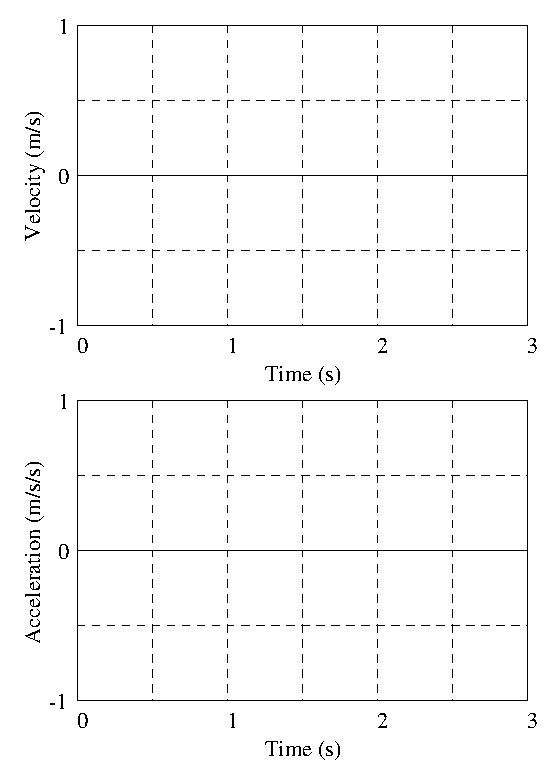
\includegraphics{slowing/slowing_fig1.eps} \par}
%\vspace{0.3cm}
\begin{lab_groupplot}*{}[lab_grid,
	group style={
		group size=1 by 2,
		xlabels at=edge bottom,
		vertical sep=0.4in,
		},
	width=4.5in,  height=1.8in,
	xlabel=Time (s),
	xmin=0, xmax=5,
	xtick distance = 1, 
	ytick distance = 1, 
	minor tick num=1
	]
\nextgroupplot[
	ymin=-1,ymax=1, 
	ylabel={Velocity (m/s)},
	]
\nextgroupplot[
	ymin=-1,ymax=1, 
	ylabel={Acceleration (m/s$^2$)},
	]
\end{lab_groupplot}

(b) To test your predictions, open the \filename{P\_V\_A\_Graphs.cap} application in the \filename{\coursefolder} folder. Turn on the cart at your station and connect it to the computer via Bluetooth. You may need to zero (or tare) the built-in acceleration sensor. Use the lab stand to raise the track several centimeters at one end. Give the cart a gentle push near the lowered end of the track and create graphs of its motion as it moves in the positive direction (defined by the $x$-axis printed on the top of the cart) up the incline. Stop the cart before it turns around or hits the end of the track. Sketch the graphs neatly on the above axes using solid lines. The acceleration \textit{vs.}~time graphs may exhibit small fluctuations due to irregularities in the motion of the cart. You should ignore these fluctuations and draw smooth patterns.

(c) Did the shapes of your velocity and acceleration graphs agree with your predictions? How is the sign of the acceleration represented on a velocity \textit{vs.}~time graph? 
\answerspace{15mm}

(d) How is the sign of the acceleration represented on an acceleration \textit{vs.}~time
graph? 
\answerspace{15mm}

\pagebreak[3]
(e) Is the sign of the acceleration what you predicted? How does slowing down while moving in the positive direction result in this sign of acceleration? Hint: Remember that acceleration is the rate of change of velocity. Look at how the velocity is changing.
\answerspace{20mm}

%\textbf{Constructing Acceleration Vectors for Slowing Down }
\textbf{Activity 2: Constructing Acceleration Vectors for Slowing Down}

Let's consider a diagrammatic representation of a cart which is slowing down
and use vector techniques to figure out the direction of the acceleration.

%\textbf{Activity 2: Vector Diagrams for Slowing Down} 

(a) The diagram that follows shows the positions of the cart at equal time intervals.
(This is like taking snapshots of the cart at equal time intervals.) At each
indicated time, sketch, and label, a vector above the cart which might represent the velocity
of the cart at that time while it is moving in the positive direction and slowing down.

\vspace{0.5cm}
%{\par\centering 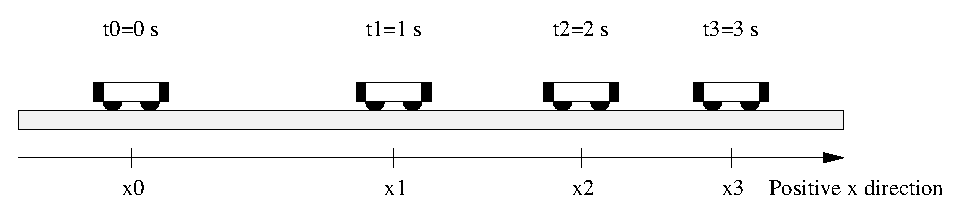
\includegraphics{slowing/slowing_fig2.eps} \par}
{\par\centering 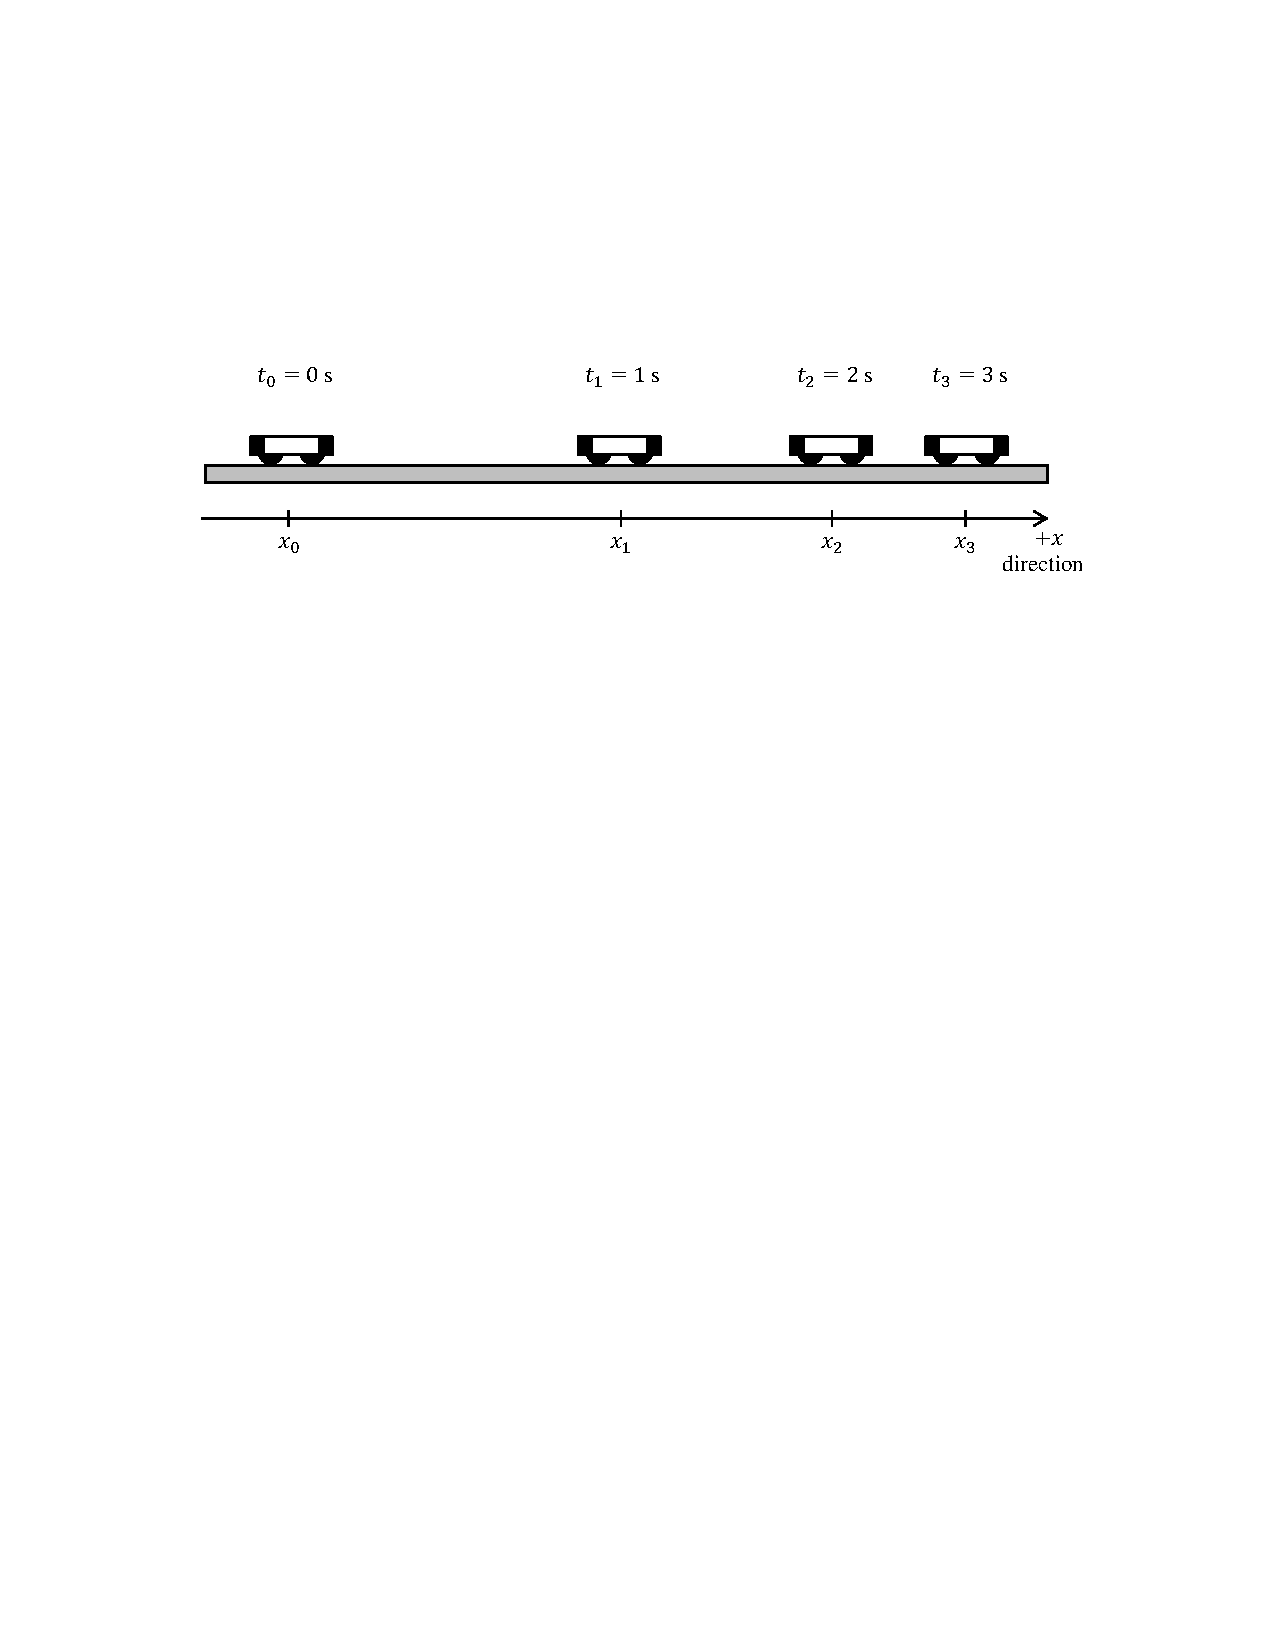
\includegraphics{slowing/carts_slowing.pdf} \par}
\vspace{0.5cm}

(b) Show below how you would find the vector representing the change in velocity
between the times $t_1 = 1$ s and $t_2 = 2$ s by creating a vector diagram using the vectors above. Based on the direction of the resultant vector and the direction of the positive $x$-axis, what is the sign of the acceleration? Does this agree with your answer to Question (e) in Activity 1?
\answerspace{25mm}

(c) By filling in the following table, state the general rules to predict the 
sign of the acceleration if you know the sign of the velocity (i.e., the 
direction of motion) and whether the object is speeding up or slowing down. 
Positive velocities have been investigated in this experiment and the previous 
one. Negative velocities we investigate below, so these are essentially 
predictions.

\vspace{0.3cm}
{\centering \begin{tabular}{|c|c|c|}
\hline
Velocity&
&
Acceleration\\
\hline
positive&
speeding up&
\\
\hline
positive&
slowing down&
\\
\hline
negative&
speeding up&
\\
\hline
negative&
slowing down&
\\
\hline
\end{tabular}\par}
\vspace{0.3cm}


%\newpage
\pagebreak[2]
\textbf{Activity 3: Speeding Up While Moving in the Negative Direction} 

(a) Predict the shape of the velocity and acceleration \textit{vs.}~time graphs
for a cart moving in the negative direction while speeding up at a constant rate. Sketch your predictions on the following axes using dashed lines.

%\vspace{0.3cm}
%{\par\centering 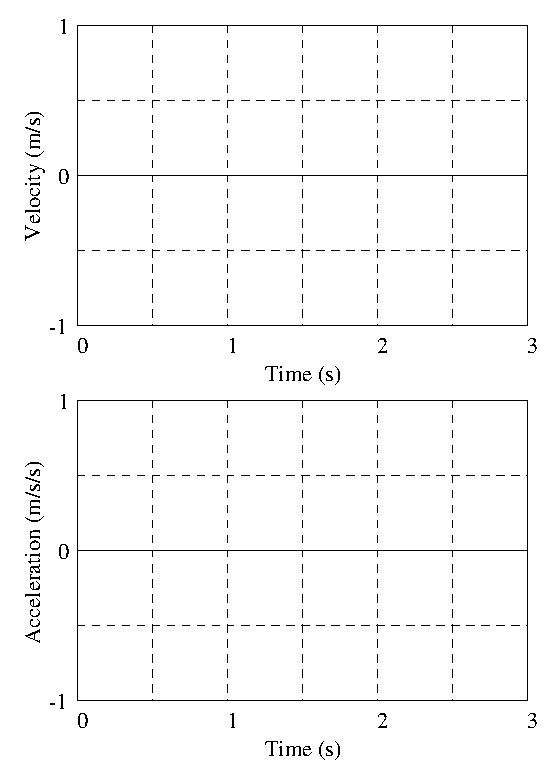
\includegraphics{slowing/slowing_fig1.eps} \par}
%\vspace{0.3cm}
\begin{lab_groupplot}*{}[lab_grid,
	group style={
		group size=1 by 2,
		xlabels at=edge bottom,
		vertical sep=0.4in,
		},
	width=4.5in,  height=1.8in,
	xlabel=Time (s),
	xmin=0, xmax=5,
	xtick distance = 1, 
	ytick distance = 1, 
	minor tick num=1
	]
\nextgroupplot[
	ymin=-1,ymax=1, 
	ylabel={Velocity (m/s)},
	]
\nextgroupplot[
	ymin=-1,ymax=1, 
	ylabel={Acceleration (m/s$^2$)},
	]
\end{lab_groupplot}

(b) To test your predictions, release the cart from rest near the raised end of the track. The cart should be oriented so that the positive direction (the $x$-axis printed on the top of the cart) points up the incline, so that the cart's motion is in the negative direction. Stop the cart before it hits the end of the track. Sketch the graphs neatly on the above axes using solid lines.

(c) How does your velocity graph show that the cart was moving in the negative direction? 
\answerspace{20mm}

(d) During the time that the cart was speeding up, is the acceleration positive
or negative? Does this agree with your prediction? Explain how speeding up while
moving in the negative direction results in this sign of acceleration. Hint: Think
about how the velocity is changing.
\answerspace{20mm}

\pagebreak[2]
\textbf{Activity 4: Constructing Acceleration Vectors for Speeding Up} 

Let's consider a diagrammatic representation of a cart which is speeding up
and use vector techniques to figure out the direction of the acceleration.

(a) The diagram that follows shows the positions of the cart at equal time intervals.
(This is like taking snapshots of the cart at equal time intervals.) At each
indicated time, sketch, and label, a vector above the cart which might represent the velocity
of the cart at that time while it is moving in the negative direction and speeding up.

%\vspace{0.3cm}
%{\par\centering 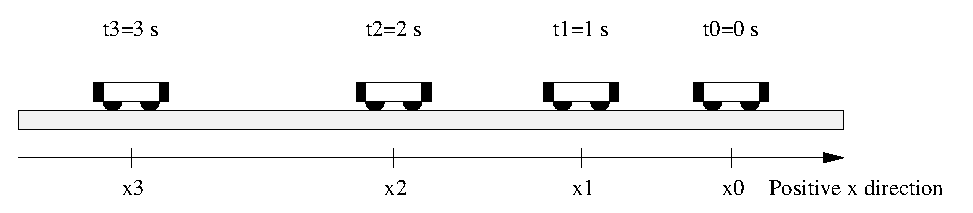
\includegraphics{slowing/slowing_fig3.eps} \par}
{\par\centering 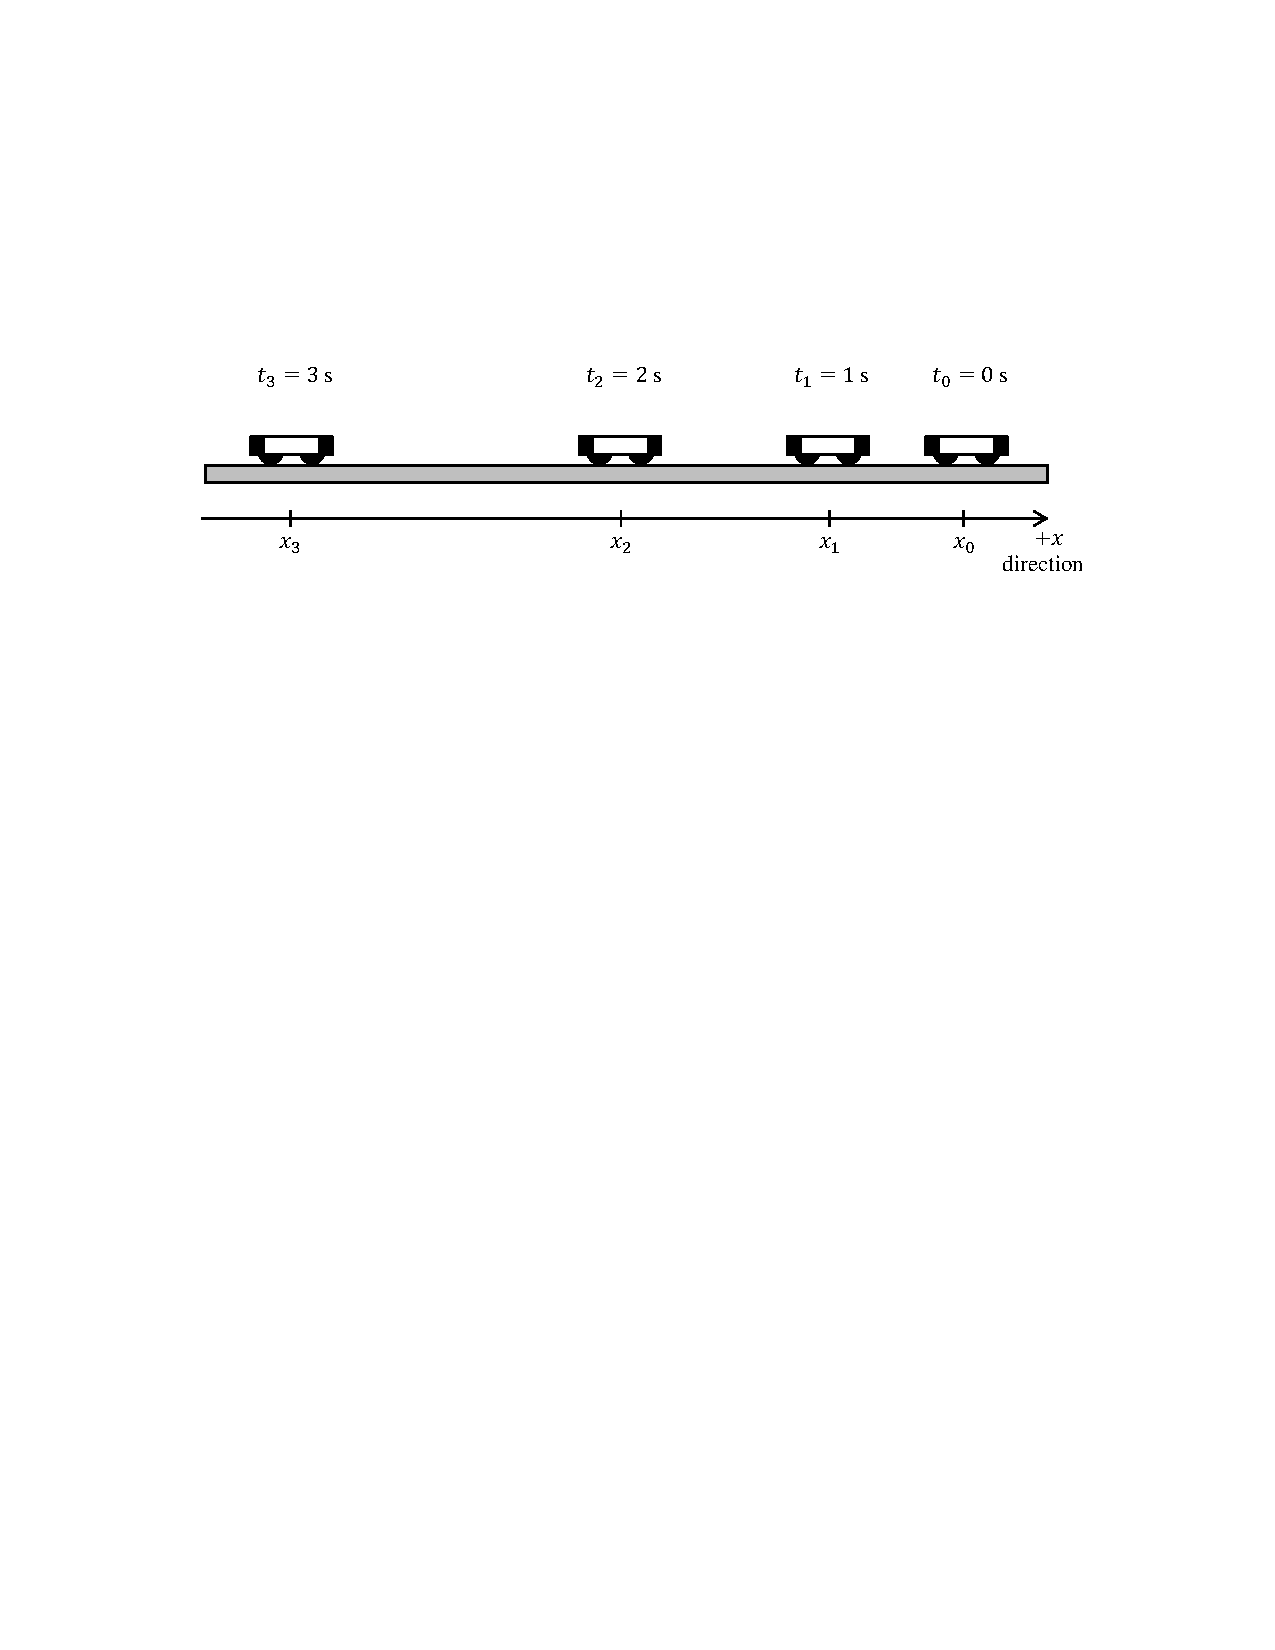
\includegraphics{slowing/carts_speeding.pdf} \par}
%\vspace{0.3cm}

(b) Show below how you would find the vector representing the change in velocity
between the times $t_1 = 1$ s and $t_2 = 2$ s as you did in Activity 2(b). Based on the 
direction of the resultant vector and the direction of the positive $x$-axis, 
what is the sign of the acceleration? Does this agree with your answer to Question (d) in Activity 3?
\vspace{20mm}

\textbf{Activity 5: Slowing Down While Moving in the Negative Direction}

There is one more possible combination of velocity and acceleration for the
cart, that of moving in the negative direction while slowing down. 

%Slowing Down Toward the Detector} 

(a) Use your general rules to predict the direction and sign of the acceleration
when the cart is slowing down as it moves in the negative direction. Explain why the
acceleration should have this sign in terms of the velocity and how the 
velocity is changing. 
\answerspace{15mm}

(b) The diagram below shows the positions of the cart at equal time intervals
for slowing down while moving in the negative direction. At each indicated time, 
sketch, and label, a vector above the cart which might represent the velocity of the cart at that time while it is moving in the negative direction and slowing down.

%\vspace{0.3cm}
%{\par\centering 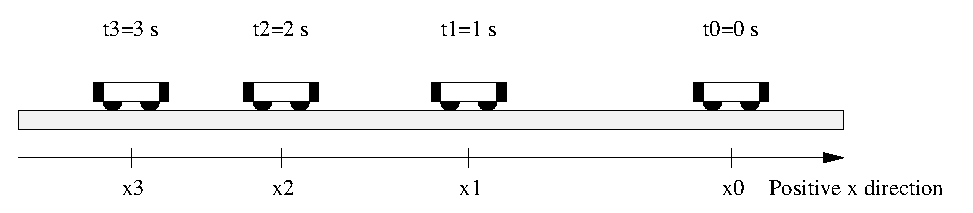
\includegraphics{slowing/slowing_fig4.eps} \par}
{\par\centering 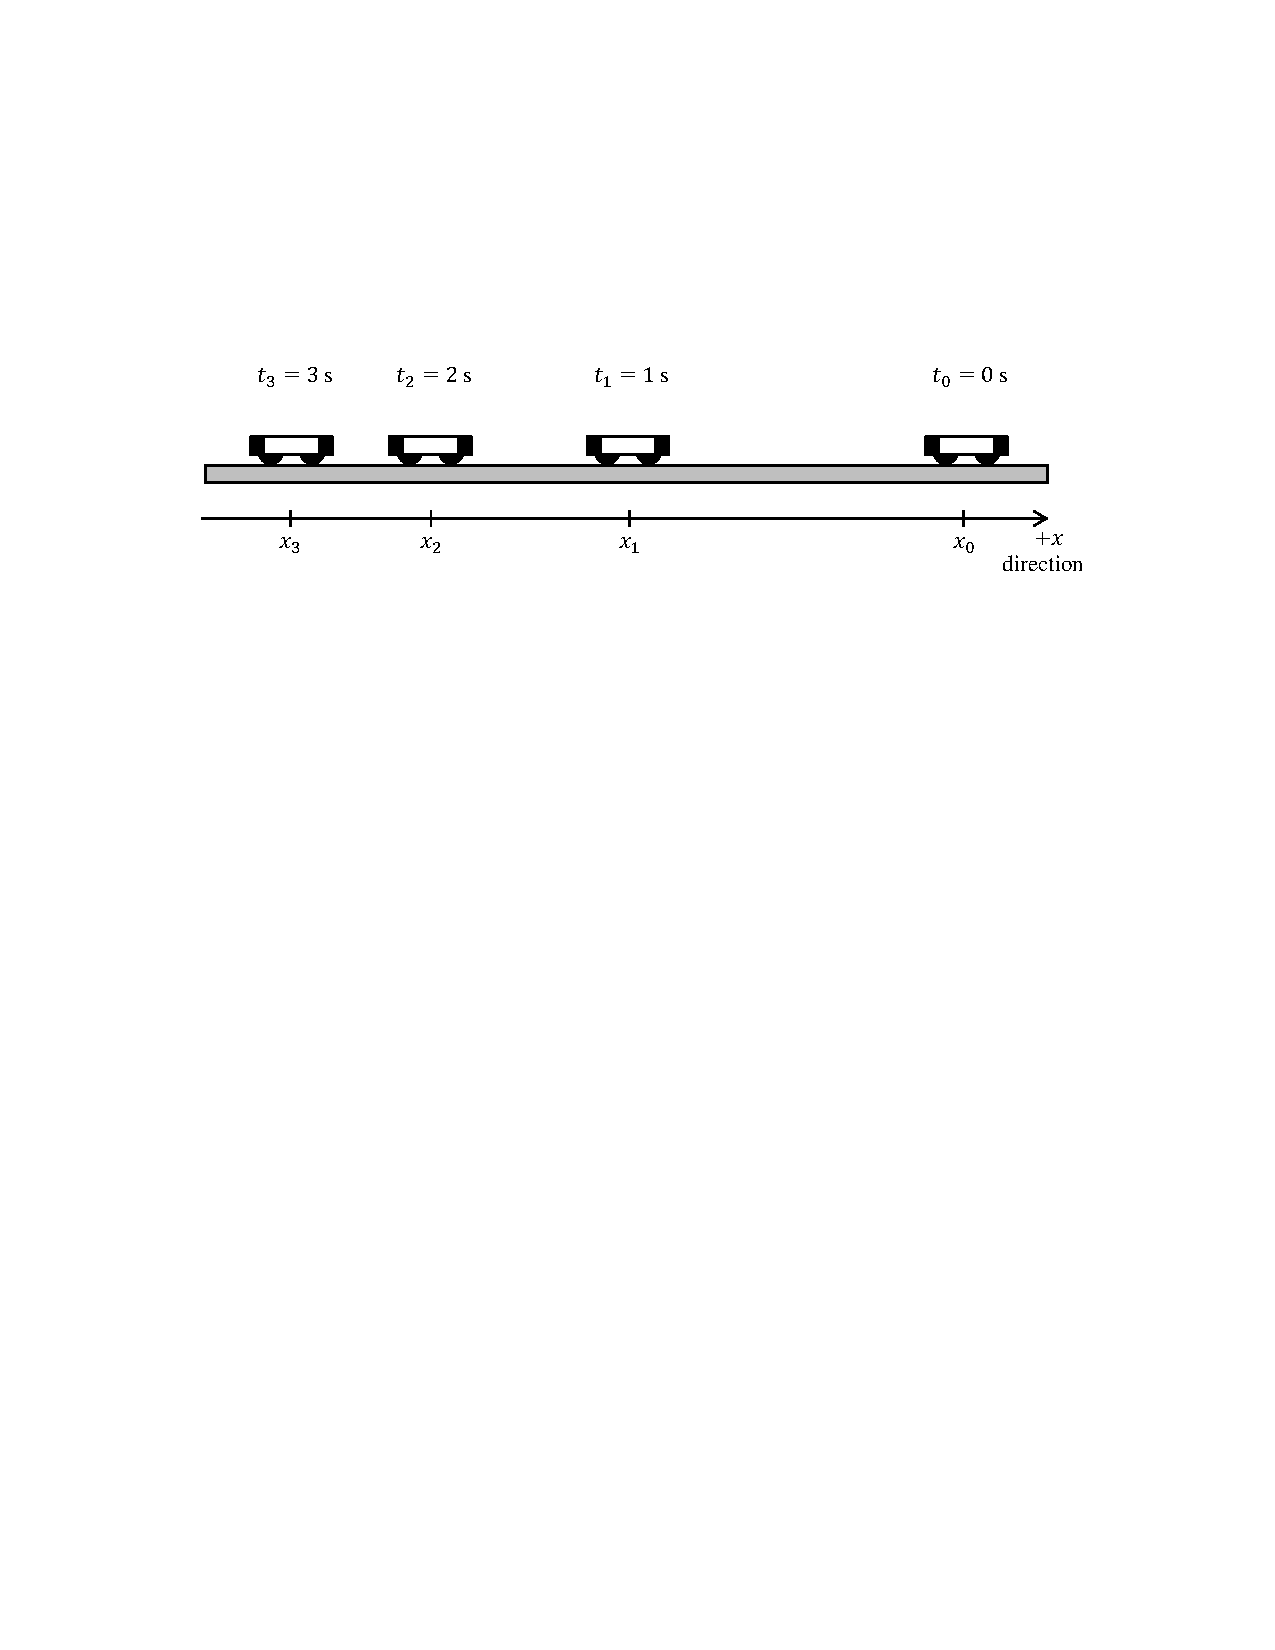
\includegraphics{slowing/carts_slowing2.pdf} \par}
%\vspace{0.3cm}

(c) Show below how you would find the vector representing the change in velocity
between the times $t_1 = 1$ s and $t_2 = 2$ s as you did in Activity 2(b). Based on the 
direction of the resultant vector and the direction of the positive $x$ axis, 
what is the sign of the acceleration?  Does this agree with the prediction you made in part (a)?
\answerspace{10mm}

\pagebreak[2]
\textbf{Activity 6: Acceleration and Turning Around }

In Lab \ref{changing_motion}, and in Activity 1 in this session, you looked at
velocity \textit{vs.}~time and acceleration \textit{vs.}~time graphs for a cart moving in one
direction with a changing velocity. In this investigation you will look at what
happens when the cart slows down, turns around and then speeds up. (This is a
combination of Activities 1 and 3.)

To practice this motion you should position the cart near the lowered end of the track and
and give the cart a gentle push in the positive direction (defined by the $x$-axis printed on the top of the cart) up the incline. It should move up the track, slow down, reverse direction and then move back down the incline. Be sure that the cart does not hit the end of the track before it turns around. Try it, but don't record the data (yet).
%\textbf{Activity 6: Reversing Direction }

(a) For each part of the motion (up the incline, at the turning point,
and down the incline) predict in the table that follows whether the cart's velocity
is positive, zero or negative. Also indicate whether the acceleration is
positive, zero or negative.

\vspace{0.3cm}
{\centering \begin{tabular}{|c|c|c|c|}
\hline 
&
Moving Away&
Turning Around&
Moving Toward\\
\hline 
Velocity&
&
&
\\
\hline 
Acceleration&
&
&
\\
\hline 
\end{tabular}\par}
\vspace{0.3cm}

(b) Sketch the predicted shapes of the velocity \textit{vs.}~time and acceleration 
\textit{vs.}~time graphs of this entire motion on the axes that follow using dashed lines.

%\vspace{0.3cm}
%{\par\centering 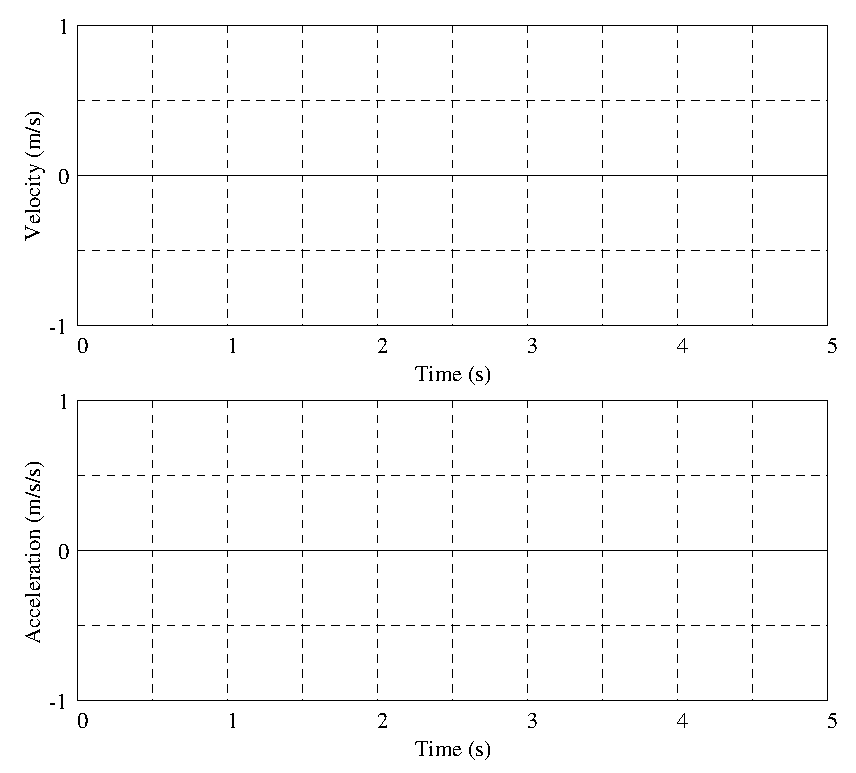
\includegraphics{slowing/slowing_fig5.eps} \par}
%\vspace{13mm}
\begin{lab_groupplot}*{}[lab_grid,
	group style={
		group size=1 by 2,
		xlabels at=edge bottom,
		vertical sep=0.4in,
		},
	width=4.5in,  height=1.8in,
	xlabel=Time (s),
	xmin=0, xmax=5,
	xtick distance = 1, 
	ytick distance = 1, 
	minor tick num=1
	]
\nextgroupplot[
	ymin=-1,ymax=1, 
	ylabel={Velocity (m/s)},
	]
\nextgroupplot[
	ymin=-1,ymax=1, 
	ylabel={Acceleration (m/s$^2$)},
	]
\end{lab_groupplot}

(c) Test your predictions by making graphs of the motion. Use the procedures
you used in the slowing down and speeding up activities. You may have to try
a few times to get a good run. When you get a good run, sketch both graphs on the axes above using solid lines.

\pagebreak[2]
(d) Did the cart have a zero velocity at any point in the motion? Does this agree with your prediction? How much time did it spend at zero velocity?
\answerspace{20mm}

(e) According to your acceleration graph, what is the acceleration at the instant
the cart comes to rest? Is it positive, negative or zero? Does this agree with
your prediction? 
\answerspace{20mm}

(f) Explain the observed sign of the acceleration when the cart changes direction. (Hint: Remember that acceleration is the rate of change of velocity.) 
\answerspace{20mm}

(g) If your instructor requests it, print a copy of the position, velocity, and acceleration graphs for each person.

(h) Notice that the slope of the velocity graph is not quite the same for positive velocities as it is for negative velocities. (This difference can also be seen on the acceleration graph.) What accounts for this difference?
\answerspace{20mm}

%\textbf{Tossing a Ball }
\textbf{Activity 7: The Rise and Fall of a Ball} 

Suppose you throw a ball up into the air. It moves upward, reaches its highest
point and then moves back down toward your hand. We will now consider what can be said about the directions of its velocity and acceleration vectors at various points.

(a) Consider the ball toss carefully. Assume that upward is the positive direction.
Indicate in the table that follows whether the velocity is positive, zero or
negative during each of the three parts of the motion. Also indicate if the
acceleration is positive, zero or negative. Hint: Remember, to find the acceleration
you must look at the change in velocity.

\vspace{0.3cm}
{\centering \begin{tabular}{|c|c|c|c|}
\hline 
&
Moving Up&
At Highest Point&
Moving Down\\
&
(After Release)&
&
\\
\hline 
Velocity&
&
&
\\
\hline 
Acceleration&
&
&
\\
\hline 
\end{tabular}\par}
\vspace{0.3cm}

(b) In what ways is the motion of the ball similar to the motion of the cart
which you just observed?
\answerspace{10mm}

\pagebreak[3]
\textbf{Homework} 

1. An object moving along a line (the + position axis) has the acceleration-time graph below. How might the object move to create this graph if it is moving
\emph{toward the origin}?

%\vspace{0.3cm}
%{\par\centering 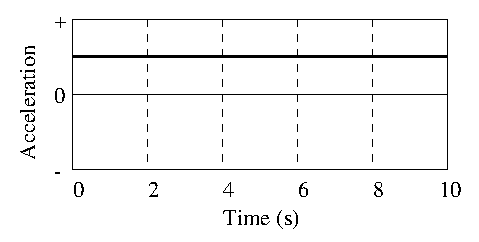
\includegraphics{slowing/slowing_fig6.eps} \par}
%\vspace{0.3cm}
\begin{lab_axis}[lab_noticks_2quads,
	width=2.0in,  height=1.2in,
	plus_minus_zero_labels,
	xlabel=Time,
	ylabel=Acceleration,
	]
\addplot {0.4};
\end{lab_axis}

2. Sketch on the axes below a velocity-time graph that goes with the above
acceleration-time graph.

%\vspace{0.3cm}
%{\par\centering 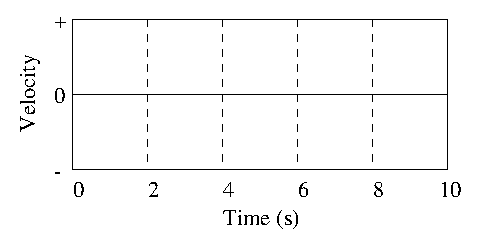
\includegraphics{slowing/slowing_fig7.eps} \par}
%\vspace{0.3cm}
\begin{lab_axis}*[lab_noticks_2quads,
	width=2.0in,  height=1.2in,
	plus_minus_zero_labels,
	xlabel=Time,
	ylabel=Velocity,
	]
\end{lab_axis}

3. How would an object move to create each of the three \emph{labeled} parts of the
acceleration-time graph shown below? (Consider the labeled horizontal line segments only, not the connectors between them.)

%\vspace{0.3cm}
%{\par\centering 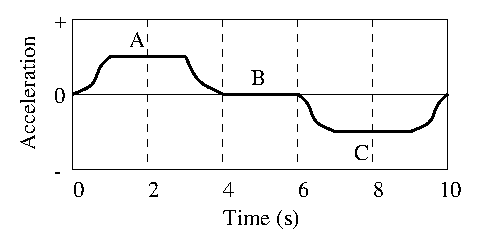
\includegraphics{slowing/slowing_fig8.eps} \par}
%\vspace{0.3cm}
\begin{lab_axis}*[lab_noticks_2quads,
	width=3.0in,  height=1.2in,
	plus_minus_zero_labels,
	xlabel=Time,
	ylabel=Acceleration,
	xmax=1.0,
	xtick={0.15,0.45,0.75},
	xticklabels={A,B,C},
	]
\addplot coordinates {(0,0) (0.02,0.5) (0.28,0.5) (0.3,0.0) (0.6,0) (0.62,-0.5) (0.88,-0.5) (0.9,0.0)};
\end{lab_axis}

\hspace{20mm}A: 
\answerspace{0.5in}

\hspace{20mm}B: 
\answerspace{0.5in}

\hspace{20mm}C:
\answerspace{0.5in}

\pagebreak[2]
4. Sketch below a velocity-time graph which might go with the acceleration-time graph in question (3). (Again, consider the straight line segments only.)

%\vspace{0.3cm}
%{\par\centering 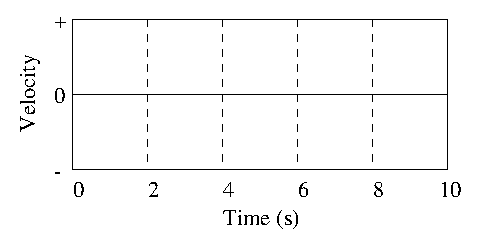
\includegraphics{slowing/slowing_fig9.eps} \par}
%\vspace{0.3cm}
\begin{lab_axis}*[lab_noticks_2quads,
	width=2.0in,  height=1.2in,
	plus_minus_zero_labels,
	xlabel=Time,
	ylabel=Velocity,
	]
\end{lab_axis}

5. Sketch the shape of the acceleration-time graph that goes with the velocity-time graph shown below.

%\vspace{0.3cm}
%{\par\centering 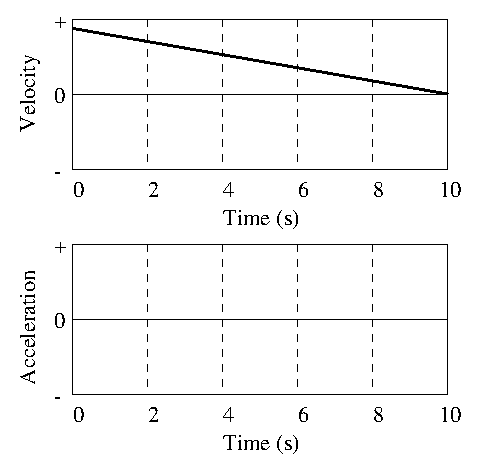
\includegraphics{slowing/slowing_fig10.eps} \par}
%\vspace{0.3cm}
\begin{lab_groupplot}*{}[lab_noticks_2quads,
	group style={group size=1 by 2},
	width=2.0in,  height=1.2in,
	plus_minus_zero_labels,
	xlabel=Time,
	]
\nextgroupplot[
	ylabel=Velocity,
	]
\addplot coordinates {(0,0.8) (0.9,0)};
\nextgroupplot[
	ylabel=Acceleration,
	]
\end{lab_groupplot}


6. A car moves along a line {[}the + position axis{]}. Fill in the table below
with the sign (+ or -) of the velocity and acceleration of the car for each
of the motions described.

\vspace{0.3cm}
{\centering \begin{tabular}{|c|c|c|c|c|}
\hline 
&
Position&
Velocity&
Acceleration&
Acceleration\\
&
&
&
Speeding Up&
Slowing Down\\
\hline 
Car Moves Away&
+&
&
&
\\
from the Origin&
&
&
&
\\
\hline 
Car Moves Toward&
+&
&
&
\\
the Origin&
&
&
&
\\
\hline 
\end{tabular}\par}
\vspace{0.3cm}

\newpage

7. For each of the position-time graphs shown, sketch below it the corresponding
velocity-time and acceleration-time graphs.

%\vspace{0.3cm}
%{\par\centering 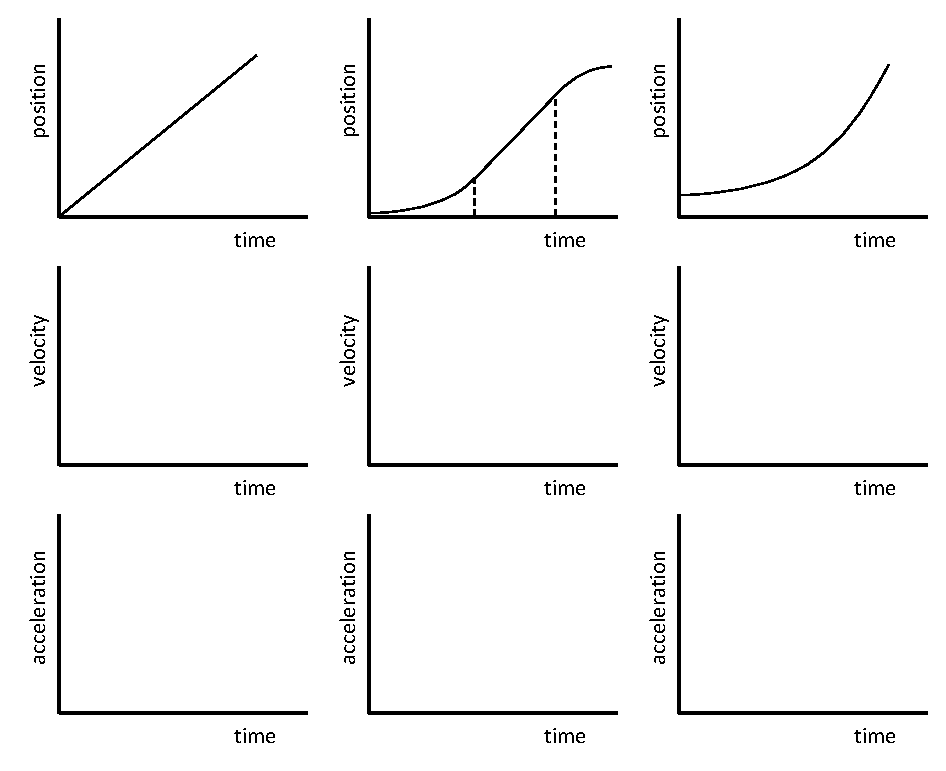
\includegraphics[width=0.85\textwidth]{slowing/slowing_fig11_new.eps} \par}
%\vspace{0.3cm}
\begin{lab_groupplot}*{}[lab_noticks_1quad,
	group style={group size=3 by 3},
	width=1.5in,  height=1.2in,
	xlabel=Time,
	]
\nextgroupplot[ylabel=Position]
	\addplot {x};
\nextgroupplot[ylabel=Position]
	\addplot{x^2 + 0.2};
\nextgroupplot[ylabel=Position]
	\addplot +[domain=0.00:0.25]{2*x^2 + 0.2};
	\addplot +[domain=0.25:0.60]{x + 0.075};
	\addplot +[domain=0.60:0.85]{-2*(x-0.85)^2 + 0.8};
	\addplot +[dashed, thick] coordinates{(0.25,0) (0.25,0.32)};
	\addplot +[dashed, thick] coordinates{(0.60,0) (0.60,0.7)};
\nextgroupplot[ylabel=Velocity]
\nextgroupplot[ylabel=Velocity]
\nextgroupplot[ylabel=Velocity]
\nextgroupplot[ylabel=Acceleration]
\nextgroupplot[ylabel=Acceleration]
\nextgroupplot[ylabel=Acceleration]
\end{lab_groupplot}

8. Describe how you would move to produce the velocity-time graph shown below.

%\vspace{0.3cm}
%{\par\raggedright 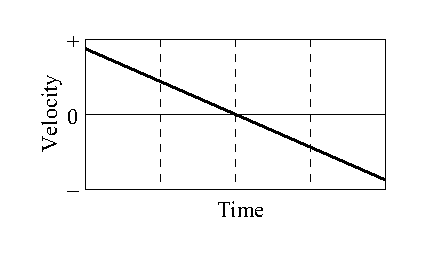
\includegraphics{slowing/slowing_fig12.eps} \par}
%\vspace{0.3cm}
\begin{lab_axis}[lab_noticks_2quads,
	width=2.0in,  height=1.2in,
	plus_minus_zero_labels,
	xlabel=Time,
	ylabel=Velocity,
	]
\addplot coordinates {(0,0.8) (0.9,-0.8)};
\end{lab_axis}

9. Sketch a position-time graph corresponding to the velocity-time graph above.

%\vspace{0.3cm}
%{\par\centering 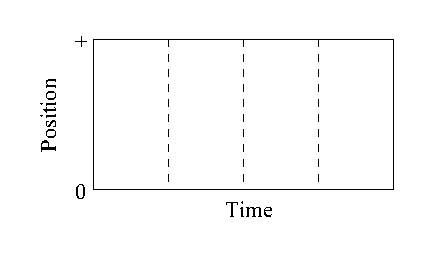
\includegraphics{slowing/slowing_fig13.eps} \par}
%\vspace{0.3cm}
\begin{lab_axis}*[lab_noticks_1quad,
	width=2.0in,  height=1.2in,
	xlabel=Time,
	ylabel=Position,
	]
\end{lab_axis}

\pagebreak
10. Sketch an acceleration-time graph corresponding to the velocity-time graph above.

%\vspace{0.3cm}
%{\par\centering 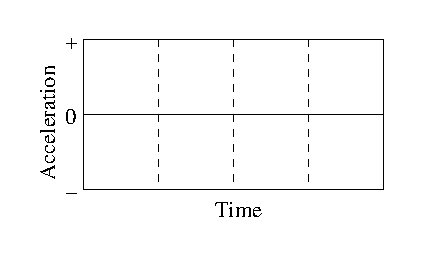
\includegraphics{slowing/slowing_fig14.eps} \par}
%\vspace{0.3cm}
\begin{lab_axis}*[lab_noticks_2quads,
	width=2.0in,  height=1.2in,
	plus_minus_zero_labels,
	xlabel=Time,
	ylabel=Acceleration,
	]
\end{lab_axis}

A car can move in either direction along a line (the + position axis). Sketch
velocity-time and acceleration-time graphs that correspond to each of the following descriptions of the car's motion.

11. The car is moving toward the origin at a constant velocity.

%\vspace{0.3cm}
%{\par\centering 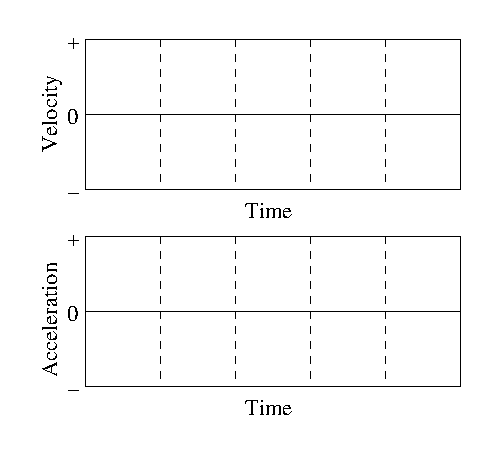
\includegraphics{slowing/slowing_fig15.eps} \par}
%\vspace{0.3cm}
\begin{lab_groupplot}*{}[lab_noticks_2quads,
	group style={group size=1 by 2},
	width=2.0in,  height=1.2in,
	plus_minus_zero_labels,
	xlabel=Time,
	]
\nextgroupplot[
	ylabel=Velocity,
	]
\nextgroupplot[
	ylabel=Acceleration,
	]
\end{lab_groupplot}

12. The car starts from rest and moves toward the origin, speeding up at a steady
rate.

%\vspace{0.3cm}
%{\par\centering 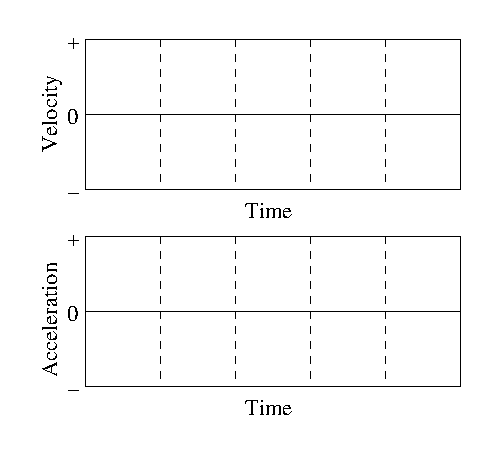
\includegraphics{slowing/slowing_fig15.eps} \par}
%\vspace{0.3cm}
\begin{lab_groupplot}*{}[lab_noticks_2quads,
	group style={group size=1 by 2},
	width=2.0in,  height=1.2in,
	plus_minus_zero_labels,
	xlabel=Time,
	]
\nextgroupplot[
	ylabel=Velocity,
	]
\nextgroupplot[
	ylabel=Acceleration,
	]
\end{lab_groupplot}

13. A ball is tossed in the air. It moves upward, reaches its highest point
and falls back downward. Sketch a velocity-time and an acceleration-time graph for the ball from the moment it leaves the thrower's hand until the moment just before it reaches their hand again. Consider the positive direction to be upward.

%\vspace{0.3cm}
%{\par\centering 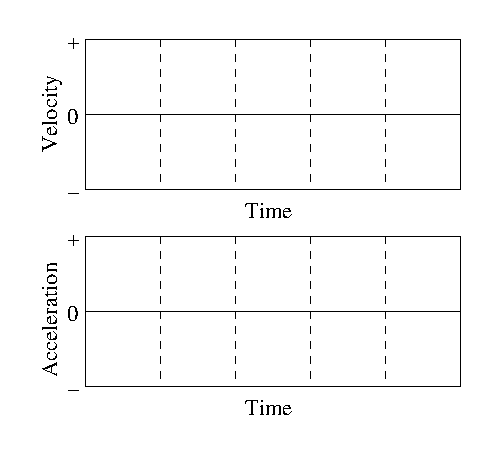
\includegraphics{slowing/slowing_fig15.eps} \par}
%\vspace{0.3cm}

\begin{lab_groupplot}*{}[lab_noticks_2quads,
	group style={group size=1 by 2},
	width=2.0in,  height=1.2in,
	plus_minus_zero_labels,
	xlabel=Time,
	]
\nextgroupplot[
	ylabel=Velocity,
	]
\nextgroupplot[
	ylabel=Acceleration,
	]
\end{lab_groupplot}

14. Each of the pictures below represents a car driving down a road. The motion
of the car is described. In each case, draw velocity and acceleration vectors
above the car which might represent the described motion. Also specify the sign
of the velocity and the sign of the acceleration. (The positive direction is toward the right.)

(a) The driver has stepped on the accelerator and the car is just starting to
move forward.

\vspace{0.3cm}
%{\par\centering 
\includegraphics{slowing/slowing_fig16.eps} \par}
{\par\centering 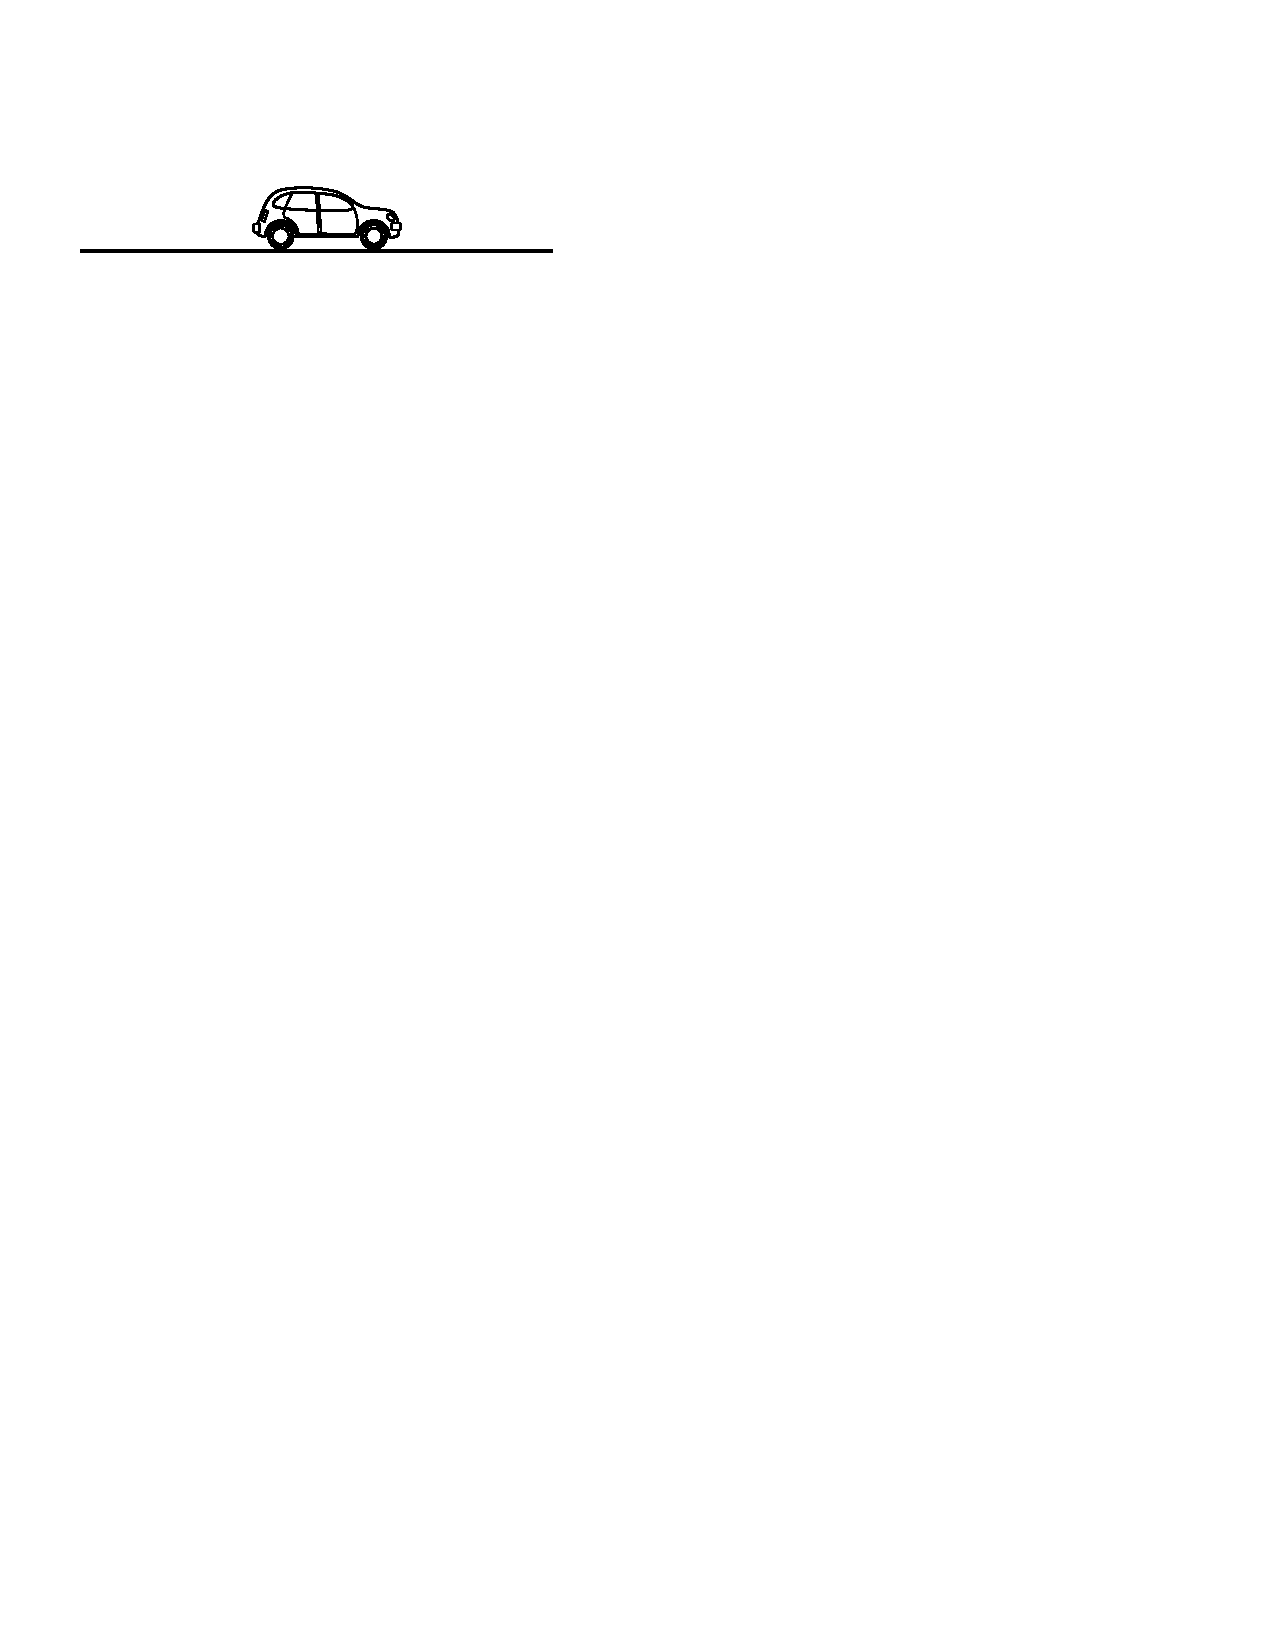
\includegraphics{slowing/car_on_ground.pdf} \par}
\vspace{0.3cm}

(b) The car is moving forward. The brakes have been applied. The car is slowing
down, but has not yet come to rest.

\vspace{0.3cm}
%{\par\centering 
\includegraphics{slowing/slowing_fig16.eps} \par}
{\par\centering 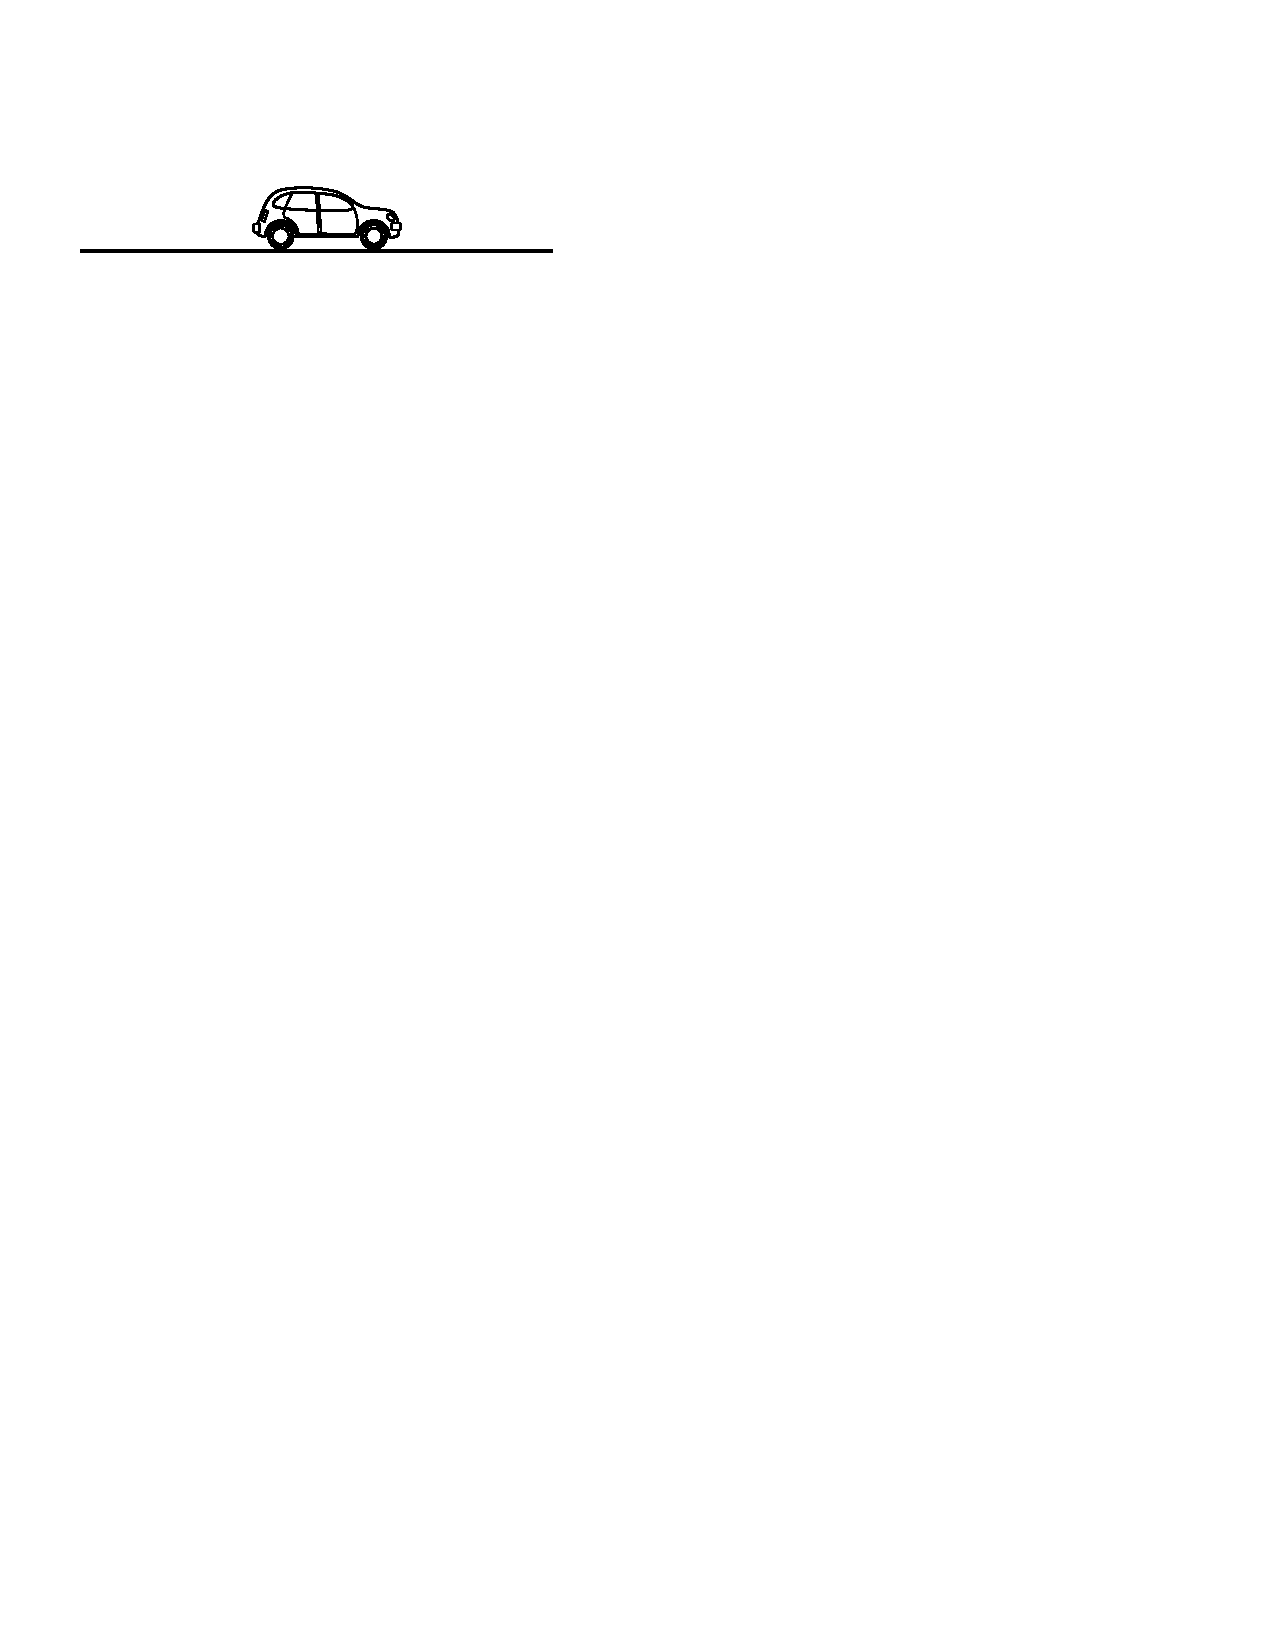
\includegraphics{slowing/car_on_ground.pdf} \par}
\vspace{0.3cm}

(c) The car is moving backward. The brakes have been applied. The car is slowing down, but has not yet come to rest.

\vspace{0.3cm}
%{\par\centering 
\includegraphics{slowing/slowing_fig16.eps} \par}
{\par\centering 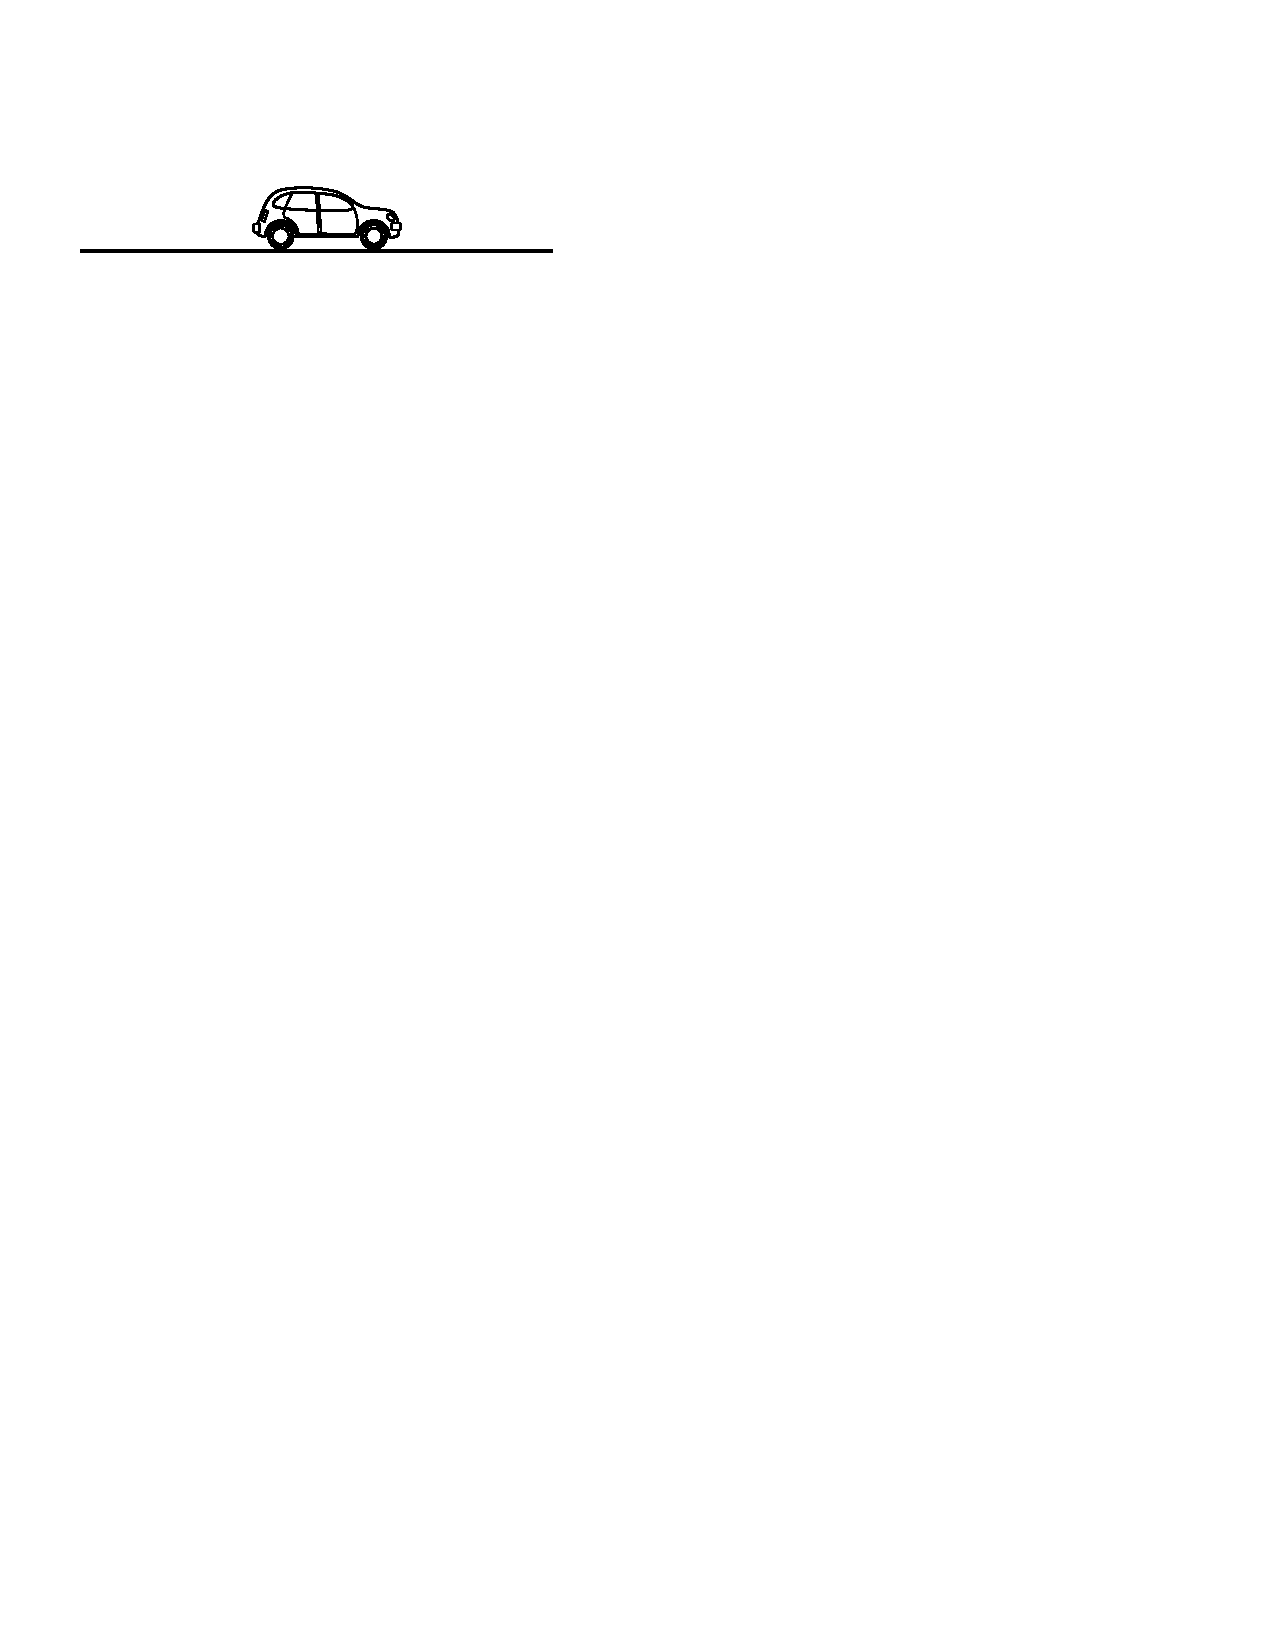
\includegraphics{slowing/car_on_ground.pdf} \par}
\vspace{0.3cm}

\newpage

The following graphs represent the motions of objects along the positive position axis. Notice that the motion of the objects is represented by position, velocity, or acceleration graphs.

Answer the following questions. You may use a graph more than once or not at
all, and there may be more correct choices than blanks. If none of the graphs
is correct, answer none.

%\vspace{0.3cm}
%{\par\centering 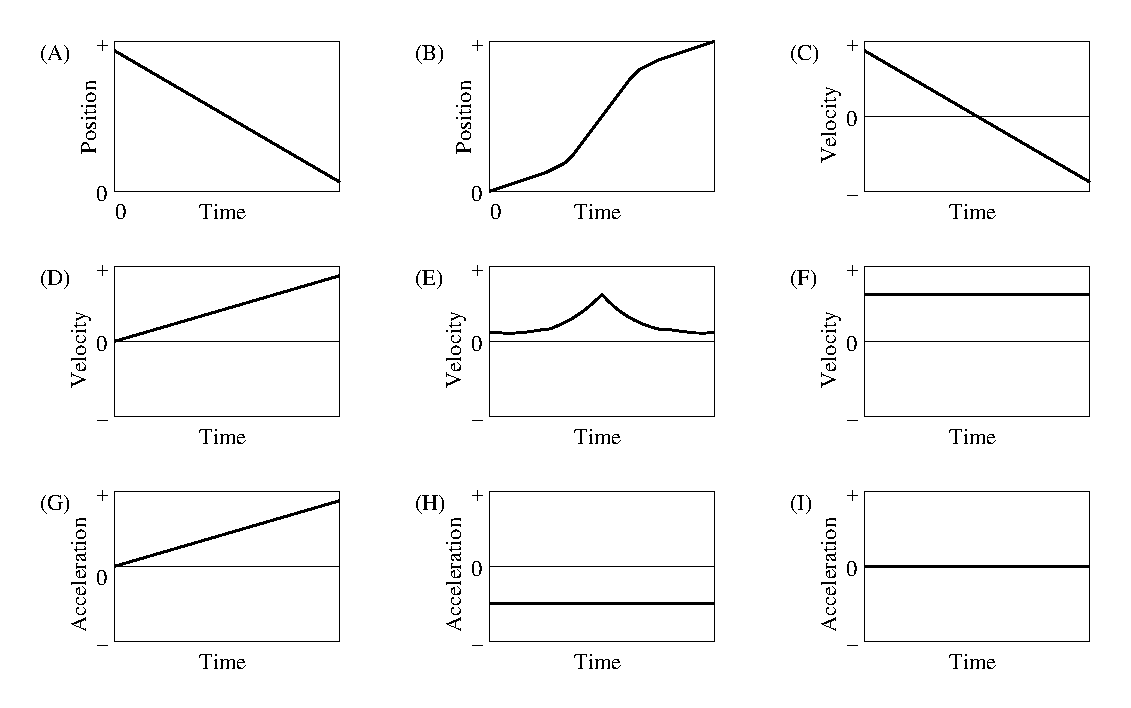
\includegraphics[trim={0.2cm 0 0.2cm 0},clip,width=\textwidth]{slowing/slowing_fig17.eps} \par}
%\vspace{0.3cm}

\begin{center}
\begin{lab_groupplot}{}[lab_noticks_2quads,
	group style={
		group size=1 by 3,
		},
	width=1.2in,  height=1.0in,
	xlabel=Time,
      title style={anchor=north},
	]
\nextgroupplot[
	lab_noticks_1quad,
	ylabel=Position,
	ylabel_align={0},
	title=(A),
	]
\addplot coordinates {(0,0.8) (0.9,0)};
\nextgroupplot[
	ylabel=Velocity,
	plus_minus_zero_labels,
	title=(D),
	]
\addplot coordinates {(0,0) (0.9,0.8)};
\nextgroupplot[
	ylabel=Acceleration,
	plus_minus_zero_labels,
	title=(H),
	]
\addplot coordinates {(0,0) (0.9,0.8)};
\end{lab_groupplot}
\begin{lab_groupplot}{}[lab_noticks_2quads,
	group style={
		group size=1 by 3,
		},
	width=1.2in,  height=1.0in,
	xlabel=Time,
      title style={anchor=north},
	]
\nextgroupplot[
	lab_noticks_1quad,
	ylabel=Position,
	ylabel_align={0},
	title=(B),
	]
\addplot coordinates {(0,0) (0.3,0.1) (0.6,0.7) (0.9,0.8)};
\nextgroupplot[
	ylabel=Velocity,
	plus_minus_zero_labels,
	title=(E),
	]
\addplot +[domain=0:0.46] {2.2*x^2 + 0.2};
\addplot +[domain=0.45:0.9] {2.2*(x-0.9)^2 + 0.2};
\nextgroupplot[
	ylabel=Acceleration,
	plus_minus_zero_labels,
	title=(G),
	]
\addplot {-0.4};
\end{lab_groupplot}
\begin{lab_groupplot}{}[lab_noticks_2quads,
	group style={
		group size=1 by 3,
		},
	width=1.2in,  height=1.0in,
	xlabel=Time,
      title style={anchor=north},
	plus_minus_zero_labels,
	]
\nextgroupplot[
	ylabel=Velocity,
	ylabel_align={0},
	title=(C),
	]
\addplot coordinates {(0,0.8) (0.9,-0.8)};
\nextgroupplot[
	ylabel=Velocity,
	title=(F),
	]
\addplot {0.4};
\nextgroupplot[
	ylabel=Acceleration,
	title=(I),
	]
\addplot {0};
\end{lab_groupplot}
\end{center}

15. Pick one graph that gives enough information to indicate that the velocity
is always negative. \rule{0.5in}{0.1pt}

Pick three graphs that represent the motion of an object whose velocity is constant.

16. \rule{0.5in}{0.1pt} 17. \rule{0.5in}{0.1pt} 18. \rule{0.5in}{0.1pt}

19. Pick one graph that definitely indicates an object has reversed direction.
\rule{0.5in}{0.1pt}

20. Pick one graph that might possibly be that of an object standing still.
\rule{0.5in}{0.1pt}

Pick 3 graphs that represent the motion of objects whose acceleration is changing.

21. \rule{0.5in}{0.1pt} 22. \rule{0.5in}{0.1pt} 23. \rule{0.5in}{0.1pt}

Pick a velocity graph and an acceleration graph that could describe the motion
of the same object during the time shown.

24. Velocity graph. \rule{0.5in}{0.1pt} 25. Acceleration graph. \rule{0.5in}{0.1pt}

